\part{From visual to textual programming}

\chap{Learning AESL from VPL programs}\label{ch.next}


Congratulations! You are an expert in programming the Thymio robot using
the \textit{Visual Programming Environment (VPL)}. Now you want to move
on and use the professional \textit{Studio Programming Environment}
(\cref{fig.studio}) and its textual programming language, the
\textit{Aseba Event Scripting Language (AESL)}.

\begin{figure}[hbt]
\begin{center}
\gr{studio}{.9}
\caption{Aseba Studio environment}\label{fig.studio}
\end{center}
\end{figure}

VPL translates graphical programs (event-actions pairs) into a textual
AESL program, which is displayed in the right-hand panel of the VPL
window (panel~6 in \cref{fig.vplgui} on page~\pageref{fig.vplgui}). This tutorial uses VPL programs
from the previous chapters of this tutorial and explains the
corresponding AESL program. You will be able to use your understanding
of the VPL program to learn the fundamental concepts of AESL
programming.

Programming in Aseba Studio is also based upon the concepts of events
and actions. Since VPL programs are translated into AESL programs,
everything you learned in this tutorial is supported in Studio, but now
you have the flexibility of a full programming language with variables,
expressions, and control statements.

When you are working with Aseba Studio, you can open VPL by clicking on
the button \bu{Launch VPL} in the \emph{Tools} tab at the bottom left of
the window. You can import VPL programs into Aseba Studio simply by
opening its file.

Sections marked $^*$ present AESL programming concepts that
go beyond what is found in the VPL projects. They can be skipped when
you first read this tutorial.

\newpage

\textbf{\large Documentation}

To learn about Aseba Studio and AESL, go to the \emph{Programming
Thymio} page at\\
\href{https://www.thymio.org/en:asebausermanual}{https://www.thymio.org/en:asebausermanual}.
You can find documentation of:

\begin{itemize}
\item The Studio programming environment.
\item The AESL programming language.
\item The interface to the Thymio robot.
(There is a reference card for the interface).
\item The native functions library supported in AESL.
\end{itemize}

There is also an archive describing interesting projects in AESL,
together with the source of proposed solutions.

\sect{The Thymio Interface}

Here is the program \p{whistles.aesl} from \cref{ch.bells} together with
part of the corresponding AESL program:
 
\begin{center}
\begin{tabular}{ll}
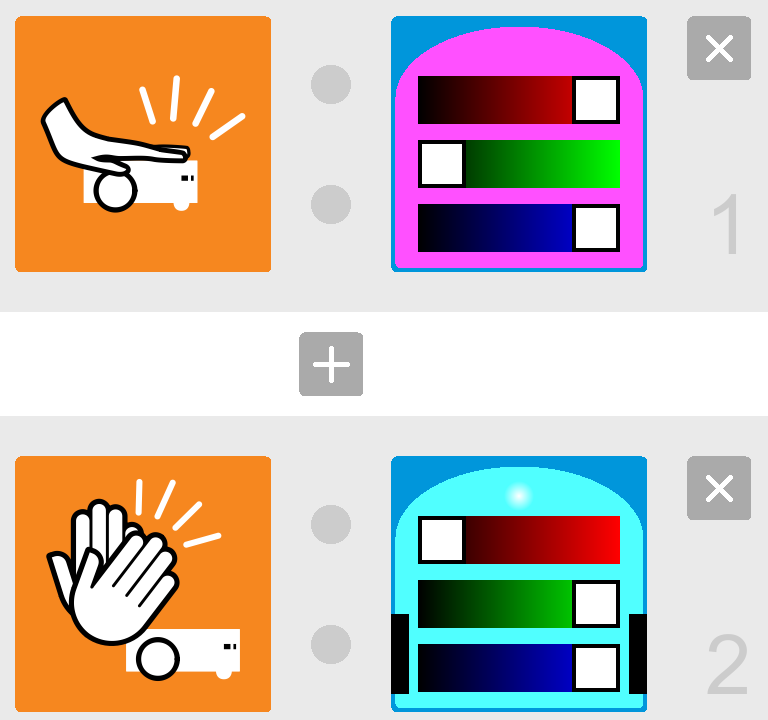
\includegraphics[width=.4\textwidth]{whistles} &
\begin{minipage}[b]{.5\textwidth}
\begin{footnotesize}
\begin{verbatim}
  onevent tap
    call leds.top(32,0,32)
  
  onevent mic
    call leds.bottom.left(0,32,32)
    call leds.bottom.right(0,32,32)
\end{verbatim}
\end{footnotesize}
\vspace*{8ex}
\end{minipage}
\end{tabular}
\end{center}

\textbf{\large Event handlers}

When a tap event occurs, the top light is turned on with the color
called \emph{magenta}, and when the clap event occurs, the bottom light
is turned on with the color called \emph{cyan}. Corresponding to the
event-actions pairs in VPL are \emph{event handlers}, which are
introduced by the keyword \p{onevent} (read this as two words: ``on
event''). You can find a list of events in the table at the bottom of
the documentation for the Thymio programming interface.

The lines following \p{onevent} form the body of the event handler
and correspond to the action blocks to the right of an event block in VPL.

When a tap event occurs, the \emph{interface function} \p{leds.top} is
\emph{called}. The function takes three \emph{parameters}, which specify
the intensities of the red, green and blue components of the LED.
Their values can range from 0 (off) to 32 (full). The combination of red
and blue gives magenta.

The VPL clap event corresponds to the \p{mic} event (short for
microphone). When the event occurs, the bottom LEDs are turned on. In
VPL, one action block turns on both LEDs to the same color, whereas in
AESL, the left and right LEDs can be set separately. Here, we set both
of them to full intensity of green and blue, giving cyan.

\textbf{\large Assigning a value to a variable}

Look again at the AESL program in the VPL window. The first two lines are:
\begin{footnotesize}
\begin{verbatim}
  # setup threshold for detecting claps
  mic.threshold = 250
\end{verbatim}
\end{footnotesize}

A line beginning with \verb+#+ is called a \emph{comment}. Comments do
not affect the running of a program; they are used to give information
to the reader of the program. Here, the comment notes that the clap
event occurs when the intensity of the sound is greater than a
\emph{threshold}. The second line of the program specifies that the
event occurs when then intensity of the sound (which can be in the range
$0$--$255$) is greater than $250$.

In VPL, the threshold is built-in and cannot be changed, but in a
textual program you can change it using an \emph{assignment statement}:
\begin{footnotesize}
\begin{verbatim}
  mic.threshold = 180
\end{verbatim}
\end{footnotesize}
Its meaning is that the \emph{value} on the right-hand side of the
\verb+=+ symbol is copied to the \emph{variable} on the left-hand side.
The variable \p{mic.threshold} is predefined for the Thymio robot.

\textbf{\large Initialization of the Thymio}

At the beginning of each program, VPL automatically inserts a sequence
of statements that turns off all the LEDs and the sound:

\begin{footnotesize}
\begin{verbatim}
  # reset outputs
  call sound.system(-1)
  call leds.top(0,0,0)
  call leds.bottom.left(0,0,0)
  call leds.bottom.right(0,0,0)
  call leds.circle(0,0,0,0,0,0,0,0)
\end{verbatim}
\end{footnotesize}

This \emph{initialization} is not visible in the VPL program. In a
textual program, it is recommended that you include these statements,
but it is not required.

\newpage

\sect{Alternatives}

The program \p{colors-multiple.aesl} from \cref{ch.colors} changes the
colors of the top and bottom LEDs when the buttons are touched:

\begin{center}
\begin{tabular}{ll}
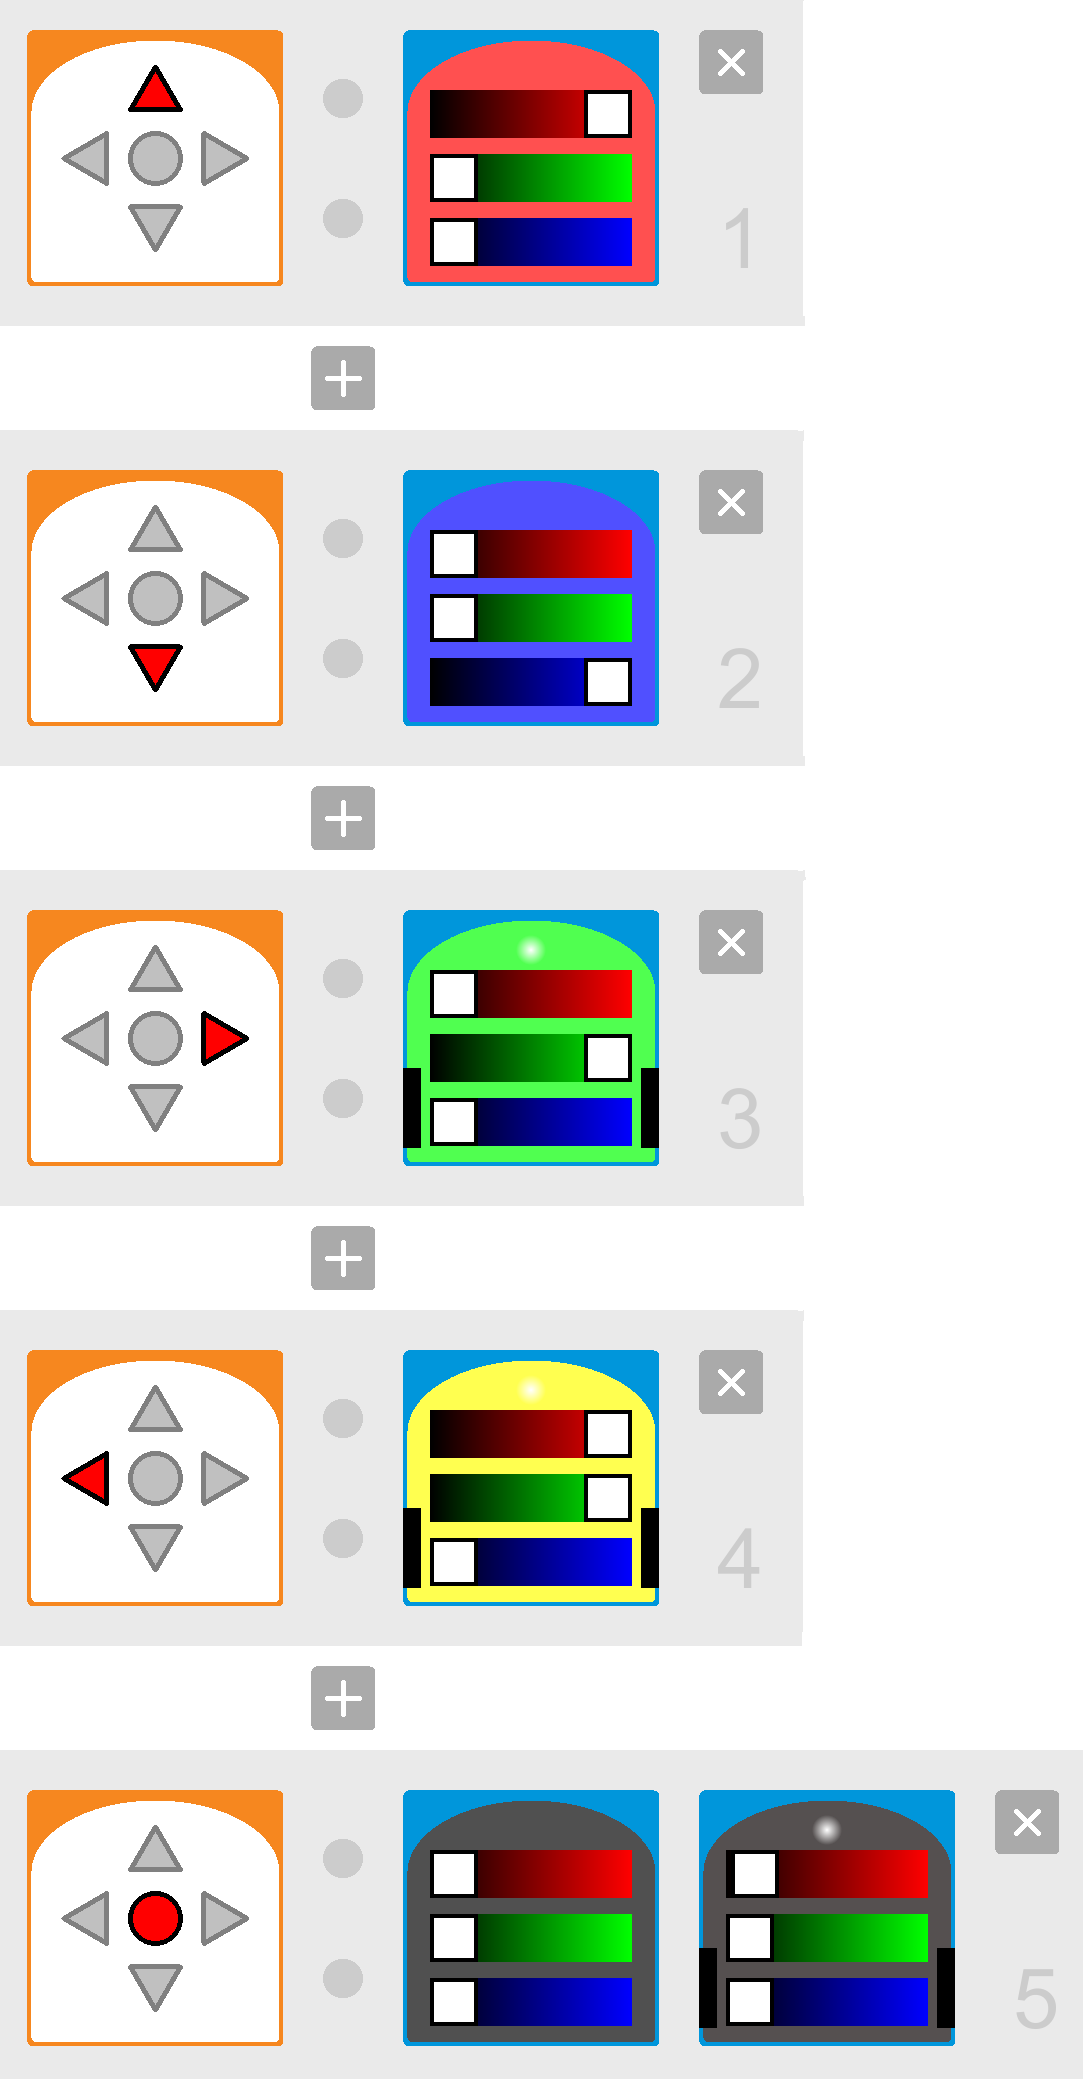
\includegraphics[width=.4\textwidth]{colors-multiple-full} &
\begin{minipage}[b]{.5\textwidth}
\begin{footnotesize}
\begin{verbatim}
  onevent buttons
    when button.forward == 1 do
      call leds.top(32,0,0)
    end
    when button.backward == 1 do
      call leds.top(0,0,32)
    end
    when button.right == 1 do
      call leds.bottom.left(0,32,0)
      call leds.bottom.right(0,32,0)
    end
    when button.left == 1 do
      call leds.bottom.left(32,32,0)
      call leds.bottom.right(32,32,0)
    end
    when button.center == 1 do
      call leds.top(0,0,0)
      call leds.bottom.left(7,0,0)
      call leds.bottom.right(7,0,0)
    end
\end{verbatim}
\end{footnotesize}
\vspace*{5ex}
\end{minipage}
\end{tabular}
\end{center}

In the AESL program, a \emph{single} event occurs when any of the five
buttons is touched. The action of the event handler \p{onevent buttons}
depends on which button is touched, so we check the value of the
\emph{button variables} in order to select an action. The statements:

\begin{footnotesize}
\begin{verbatim}
  when button.forward == 1 do
    call leds.top(32,0,0)
  end
\end{verbatim}
\end{footnotesize}

mean: \emph{when} the value of the variable \p{button.forward} changes
from some other value (here, 0) to 1, \emph{then} perform the actions
written on the lines between the keyword \p{do} and the keyword \p{end}.
There are five \p{button} variables, one for each button. The value of a
button variable is 1 if the button is touched and 0 if the button is
released. In the program, there are five \p{when}-statements, one for
each button. One or two actions are run if the expression in a
\p{when}-statement \emph{becomes} true.

\textbf{\large One event or multiple events$^*$}

The Thymio interface includes separate events for each button, in
addition to the \p{buttons} event that occurs if any button is touched
or released. We could implement the program as follows, using multiple
events without \p{when}-statements and button variables:

\begin{footnotesize}
\begin{verbatim}
  onevent button.forward
    call leds.top(32,0,0)
  
  onevent button.backward
    call leds.top(0,0,32)
  
  onevent button.right
    call leds.bottom.left(0,32,0)
    call leds.bottom.right(0,32,0)
  
  onevent button.left
    call leds.bottom.left(32,32,0)
    call leds.bottom.right(32,32,0)
  
  onevent button.center
    call leds.top(0,0,0)
    call leds.bottom.left(1,0,0)
    call leds.bottom.right(1,0,0)
\end{verbatim}
\end{footnotesize}

The advantage of using separate events is that the program is easier to
read and understand, but there are cases where you need to use the event
\p{buttons}: (a) to distinguish between touching and releasing a button,
and (b) to identify touching two buttons at once:

\begin{footnotesize}
\begin{verbatim}
  onevent buttons
    # Turn the top LEDs on when the forward button is released
    when button.forward == 0 do
      call leds.top(32,0,0)
    end

    # Turn the bottom LEDs on when
    #   both the left and the right buttons are  touched
    when button.left == 1 and button.right == 1 do
      call leds.bottom.left(0,32,0)
      call leds.bottom.right(0,32,0)
    end
\end{verbatim}
\end{footnotesize}


Another difference is that the individual events occur when a button is
touched or released, whereas the common event \p{buttons} occurs with a
frequency of 20 Hz after updating the array of button variables (see
page~\pageref{pg.hz} for an explanation of these concepts).


\textbf{\large \p{if}-statements}

AESL supports two alternative statements:
\begin{footnotesize}
\begin{verbatim}
  when v == 1 do ... statements ... end

  if v == 1 then ... statements ... end
\end{verbatim}
\end{footnotesize}
that have different meanings:
\begin{quote}
\emph{when} the value of \p{v} \emph{becomes} 1, run the statements

\emph{if} the value of \p{v} \emph{is} 1, run the statements
\end{quote}

\p{when}-statements are commonly used with variables representing
events, because we usually want to run an event handler when something
changes, not just because the value of a variable has a certain value.
We could write a \p{buttons} event handler using an \p{if}-statement:

\begin{footnotesize}
\begin{verbatim}
  onevent buttons
    if button.forward == 1 then
      ... statements ...
    end
\end{verbatim}
\end{footnotesize}
However, if we touch the forward button for a long period of time,
the statements would be run several times. If the statements change the
color of the LEDs, it wouldn't make a difference, but there are cases
where it does matter and a \p{when}-statement is needed.

An \p{if}-statement is appropriate when we are interested the values of
variables and not in their changes. The following statements set the
value of the variable \p{max} to the maximum value returned by the two
rear sensors:

\begin{footnotesize}
\begin{verbatim}
  if prox.horizontal[5] > prox.horizontal[6] then
    max = prox.horizontal[5]
  else
    max = prox.horizontal[6]
  end
\end{verbatim}
\end{footnotesize}

Additional examples of \p{if}-statements appear in the next section and
in Figure~\ref{fig.respond}.


\newpage

\sect{Arrays}

The program \p{likes.aesl} in \cref{ch.pet} of the VPL tutorial causes the
robot to follow your hand as you move it from side to side near the
forward horizontal proximity sensors.
When an object is not detected, the robot stops; when an object is
detected in front of the center sensor, the robot moves forward; when an
object is detected in front of the leftmost or rightmost sensor, the
robot turns in that direction.

\begin{figure}[hbt]
\begin{center}
\begin{tabular}{lr}
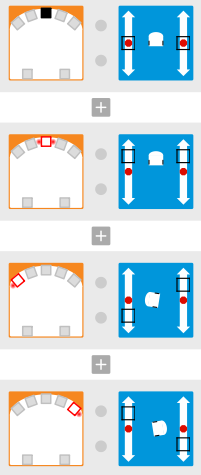
\includegraphics[width=.35\textwidth]{likes} &
\begin{minipage}[b]{.4\textwidth}
\begin{footnotesize}
\begin{verbatim}
  onevent prox
    when prox.horizontal[2] < 1000 do
      motor.left.target = 0
      motor.right.target = 0
    end
    when prox.horizontal[2] > 2000 do
      motor.left.target = 300
      motor.right.target = 300
    end
    when prox.horizontal[0] > 2000 do
      motor.left.target = -300
      motor.right.target = 300
    end
    when prox.horizontal[4] > 2000 do
      motor.left.target = 300
      motor.right.target = -300
    end
\end{verbatim}
\end{footnotesize}
\end{minipage}
\end{tabular}
\caption{The \p{likes} program in VPL and AESL}\label{fig.arrays}
\end{center}
\end{figure}

The AESL program (\cref{fig.arrays}) is structured as an event handler
with several \p{when}-statements. The values of the motor variables
\p{motor.left.target} and \p{motor.right.target} are set to values
corresponding to the positions of the sliders in the motor blocks. In
VPL, the sliders change the values of the motor variables in increments
of $50$, but in AESL you can set them to any values in the range $-500$
to $500$.

The event is called \p{prox}. Unlike the button events, which
occur when something ``happens,'' this event occurs \emph{10 times
>>>>>>> d0c474117e88c10d57f1a02945d63994237a9e8e
every second}. Before the event occurs, the values of the
\p{prox.horizontal} variables are set to values that depend on what the
sensors are detecting. See the\label{pg.hz} documentation of the
Thymio programming interface for details.\footnote{The unit
for \emph{frequency}, the number of times something happens per second, is called
the \emph{hertz}, abbreviated \emph{Hz}. The interface document specifies
that the {\footnotesize\p{prox}} event occurs with frequency \emph{10 Hz}.}

\textbf{\large Arrays as multiple variables}

The Thymio robot has 7 horizontal proximity sensors, 5 in front and 2 in
the back. To read the values detected by the sensors, it would be
possible to define 7 different variables:

\begin{footnotesize}
\begin{verbatim}
  prox.horizontal.front.0
  prox.horizontal.front.1
  prox.horizontal.front.2
  prox.horizontal.front.3
  prox.horizontal.front.4
  prox.horizontal.back.0
  prox.horizontal.back.1
\end{verbatim}
\end{footnotesize}

Instead, AESL enables you to define an \emph{array}, which is a sequence
of variables all with the same name. The different variables in the
sequence are identified with a number. The array for the horizontal
proximity sensors is predefined and is called \p{prox.horizontal}:

\begin{center}
\begin{picture}(240,40)
\put(0,0){\makebox(100,20)[l]{\p{prox.horizontal}}}
\put(100,0){\framebox(140,20){}}
\multiput(120,0)(20,0){6}{\line(0,1){20}}
\put(100,20){\makebox(20,20){\p{0}}}
\put(120,20){\makebox(20,20){\p{1}}}
\put(140,20){\makebox(20,20){\p{2}}}
\put(160,20){\makebox(20,20){\p{3}}}
\put(180,20){\makebox(20,20){\p{4}}}
\put(200,20){\makebox(20,20){\p{5}}}
\put(220,20){\makebox(20,20){\p{6}}}
\end{picture}
\end{center}

The first 5 components are for the front sensors from left to right,
while the last two components are for the back sensors from left to
right. If you don't remember the assignment of numbers to sensors, you
can always look it up in the the documentation for the Thymio
programming interface, even better, on the diagram in the reference
card.

To access a specific component in an array, write its sequence number in
square brackets after the name of the array variable. This number is
called an \emph{index} into the array. The following statement specifies
that the motor variables will be set to 300 when the value of the
\emph{front center sensor} (index 2) becomes greater than 2000:

\begin{footnotesize}
\begin{verbatim}
  when prox.horizontal[2] > 2000 do
    motor.left.target = 300
    motor.right.target = 300
  end
\end{verbatim}
\end{footnotesize}

Later, we will see that array variables can have their
values set in an assignment statement:
\begin{footnotesize}
\begin{verbatim}
  timer.period[0] = 1979
\end{verbatim}
\end{footnotesize}

\textbf{\large \p{for}-loops and index variables$^*$}

A natural generalization of arrays is to use a variable instead of a
constant for the index.\footnote{This is not used in translations of VPL
programs into AESL, except in an advanced construct for constructing
sounds; therefore, the simple example here is taken from the AESL
projects.} The program \p{cats.aesl} contains the following statements:

\begin{footnotesize}
\begin{verbatim}
  var i

  for i in 0:4 do
    if prox.horizontal[i] > DETECTION then
      state = 2
    end
  end
\end{verbatim}
\end{footnotesize}

Previously, we only used variables that are built into the Thymio
interface; here, the first line \emph{declares} a new variable called
\p{i}. The next statement is a \p{for}-statement whose meaning is:

\begin{itemize}
\item Assign the values 0, 1, 2, 3, 4 in turn to the variable \p{i};
\item For each assignment, run the statements between \p{do} and \p{end}.
\end{itemize}

Here, there is a single \p{if}-statement between \p{do} and \p{end}. It
checks the value of the horizontal proximity sensors and sets the value
2 in the variable \p{state} if the value read from a sensor is greater
than the constant \p{DETECTION}.\footnote{See the documentation of the 
Aseba Studio environment for instructions on how to define constants.}

The variable \p{i} receives the values 0, 1, 2, 3, 4 in turn, so each
time the \p{if}-statement is run, \p{prox.horizontal[i]} reads the value
of each front sensor from left to right. The result of the
\p{for}-statement is thus to set the value of the variable \p{state} to
2 \emph{if} \emph{any} of the front sensors detects an object.

\textbf{\large Declaring an array}

An array variable is declared by giving its size in brackets following
the array name. The size can also be specified by providing an initial
value:\footnote{A comment need not start at the beginning of a line.
Every character from the symbol \# to the end of the line is considered
to be a comment and is ignored by the computer.} 

\begin{footnotesize}
\begin{verbatim}
var state[4]             # An array with four components
var state[] = [0,0,0,0]  # An array with four components
\end{verbatim}
\end{footnotesize}

In the translation of the VPL program, both the size and the initial
value are given. This is correct as long as the number of values is the
same as the size:

\begin{footnotesize}
\begin{verbatim}
var state[4] = [0,0,0,0]  # OK, but redundant
\end{verbatim}
\end{footnotesize}

\newpage

\sect{Timers}

\cref{ch.time} introduced \emph{timers}. The program
\p{shy.aesl} causes the robot to turn left when the front center sensor
detects your hand; two seconds later, it turns right:

\begin{center}
\begin{tabular}{ll}
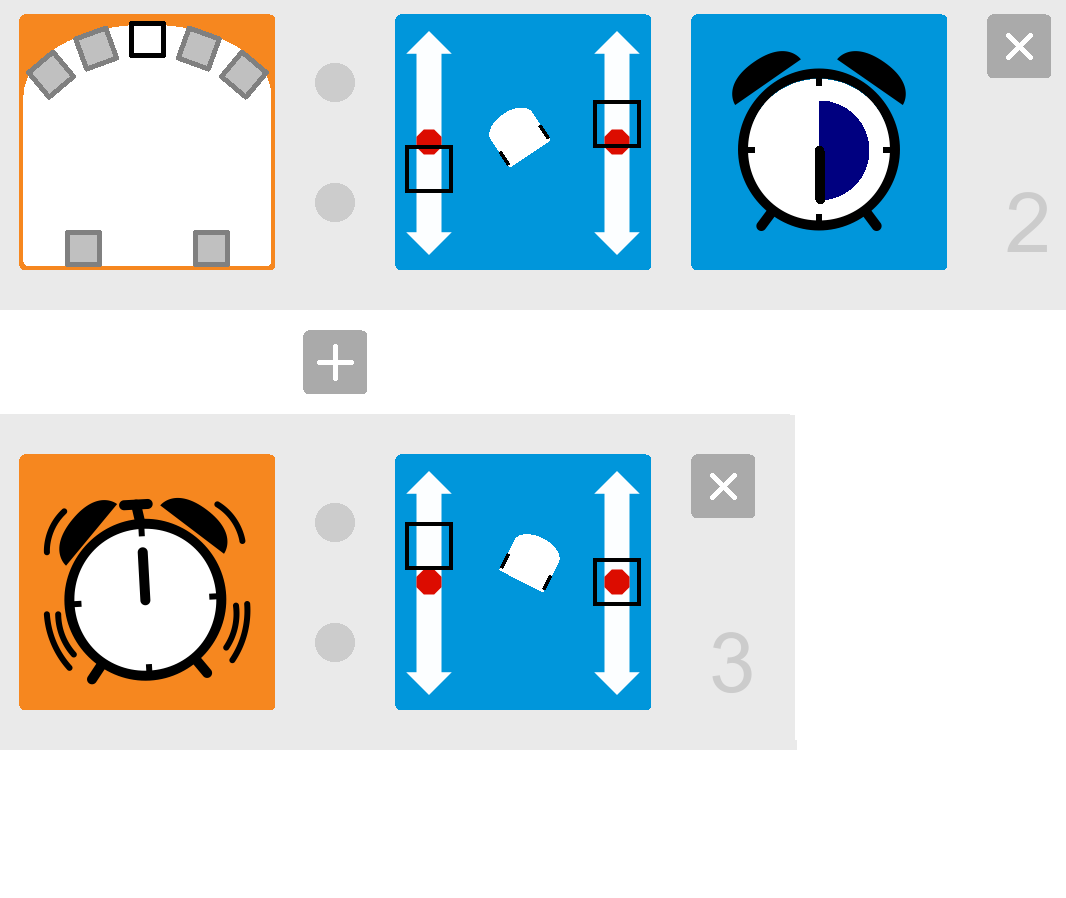
\includegraphics[width=.4\textwidth]{shy} &
\begin{minipage}[b]{.5\textwidth}
\begin{footnotesize}
\begin{verbatim}
  onevent prox
    when prox.horizontal[2] > 2000 do
      motor.left.target = -150
      motor.right.target = 100
      timer.period[0] = 2000
    end
  
  onevent timer0
    timer.period[0] = 0
    motor.left.target = 200
    motor.right.target = 0
\end{verbatim}
\end{footnotesize}
%\vspace*{1ex}
\end{minipage}
\end{tabular}
\end{center}

There are two timers in the Thymio robot. You set the duration of a
timer by assigning a value to components 0 or 1 of the array
\p{timer.period}. The value is in \emph{milliseconds}, thousandths of a
second. To set a duration of 2 seconds in timer 0, the value 2000
(milliseconds) should be assigned to \p{timer.period[0]}.

There are two events, \p{timer0} and \p{timer1}, one for each timer.
When the duration has passed (we say that the timer has \emph{expired}),
the timer event occurs. In the handler for the event \p{timer0}, we set
the timer duration to 0 so it won't occur again and change the motor
settings.

As part of its initialization, the program sets the timer to 0 so that
the event won't accidently occur at the beginning of the program:

\begin{footnotesize}
\begin{verbatim}
  # stop timer 0
  timer.period[0] = 0
\end{verbatim}
\end{footnotesize}

\newpage

\sect{States}

\cref{ch.states,ch.counting} showed how to use \emph{states}. The
Thymio robot can be in one of 16 states and you can specify that an
event causes an action only if the robot is in certain states. In the
program \p{count-to-two.aesl} from \cref{ch.counting}, the state is set to 0 when
the center button is touched and then it counts whether the number of
claps is even or odd by alternating between state 0 and state 1. The VPL
program and the AESL event handler for touching the center button
are:\footnote{The AESL program shown here is different from the one
generated by VPL as explained later in this chapter.}

\begin{center}
\begin{tabular}{ll}
\raisebox{8ex}{
\includegraphics[width=.4\textwidth]{two-button}} &
\begin{minipage}[b]{.5\textwidth}
\begin{footnotesize}
\begin{verbatim}
  var state[] = [0,0,0,0]
  
  onevent buttons
    when button.center == 1 do
      state[0] = 0
      state[1] = 0
      state[2] = 0
      state[3] = 0
    end
\end{verbatim}
\end{footnotesize}
\end{minipage}
\end{tabular}
\end{center}

The state is stored in an array \p{state[]} which has 4 components. Each
component can be 0 or 1, so there are $2\times 2\times 2\times 2=16$
possible values in the array. The components of the array are given
initial values of 0 by assigning the four values
{\footnotesize\verb+[0,0,0,0]+}. The initial value of the array is also
used to specify the number of components in an array; since there are 4
values in {\footnotesize\verb+[0,0,0,0]+}, there are 4 components in the
array.

The state event block (green, next to the button event block) has all of
its quarters set to gray; this means that the event can occur regardless
of the current value of the state. Therefore, whenever the center button
is touched, the state action block (blue) causes all the components of
the array \p{state} to be set to 0, as indicated by the white quarters.
In the corresponding AESL program, the \p{when}-statement checks if the
button was touched, but does not check the value of the array \p{state}.
If the button was touched, each component of the array is set to 0.

There are two clap event blocks, each one associated with a different
state block. In the textual program a single \p{mic} event handler will
be used. The statements to be run will depend on \p{if}-statements
(\cref{fig.respond}).

\begin{figure}[hbt]
\begin{center}
\begin{tabular}{ll}
\raisebox{10ex}{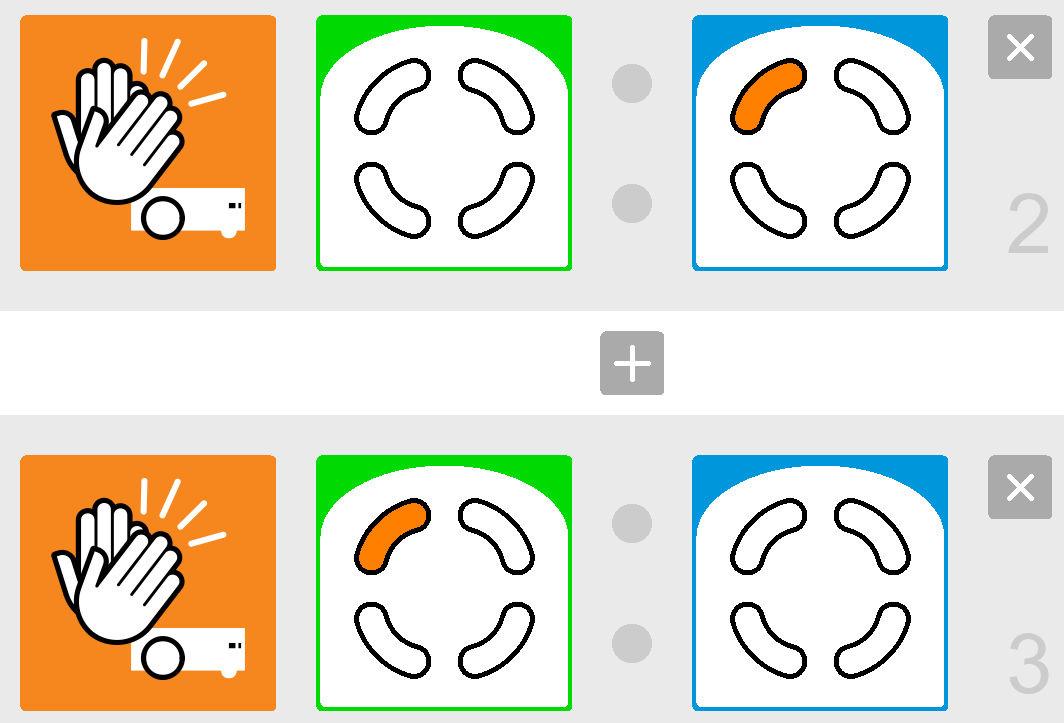
\includegraphics[width=.4\textwidth]{two-clap}} &
\begin{minipage}[b]{.5\textwidth}
\begin{footnotesize}
\begin{verbatim}
  onevent mic
    if state[0] == 0 and
       state[1] == 0 and
       state[2] == 0 and
       state[3] == 0 then
      state[0] = 1
      state[1] = 0
      state[2] = 0
      state[3] = 0
    end
    if state[0] == 1 and
       state[1] == 0 and
       state[2] == 0 and
       state[3] == 0 then
      state[0] = 0
      state[1] = 0
      state[2] = 0
      state[3] = 0
    end
\end{verbatim}
\end{footnotesize}
\end{minipage}
\end{tabular}
\caption{Responding to claps according to the state}\label{fig.respond}
\end{center}
\end{figure}

The meaning of the keyword \p{and} is that \emph{all} the conditions in
the \p{if}-statement must hold in order to run the statements between
\p{then} and \p{end}. If all components of \p{state} are 0, the value of
\p{state[0]} is set to 1, while the others are set to 0. This
corresponds to the state event block having all quarters white and the
state action block having the upper left quarter orange and the others
white. Similarly, if value of \p{state[0]} is 1 and the values of the
other components are 0, the values of all the components of \p{state}
are set to 0.

\newpage

\sect{Subroutines}

Quite often we need to run the same sequence of statements from many
places within a program. We could write the statements once and copy
them each time they are needed. A simpler solution is to use a
\emph{subroutine}, which assigns a name to a sequence of statements. In
this program, the declaration {\footnotesize\verb+sub display_state+}
declares a subroutine that assigns the name
{\footnotesize\verb+display_state+} to a sequence of statements, here,
the single statement \p{call leds.circle}:

\begin{footnotesize}
\begin{verbatim}
  # subroutine to display the current state
  sub display_state
    call leds.circle(
      0, state[1]*32, 0, state[3]*32, 0, state[2]*32, 0, state[0]*32)
\end{verbatim}
\end{footnotesize}

When the subroutine is \emph{called}, it runs the statements assigned to
the name of the subroutine:
\vspace{-1ex}
\begin{footnotesize}
\begin{verbatim}
  callsub display_state
\end{verbatim}
\end{footnotesize}
\vspace{-1ex}
The interface function \p{leds.circle} sets the eight curved LEDs
surrounding the buttons. You really do need to refer to the cheat sheet
to learn which parameter sets which LED!

The intensity of each LED is set by giving the corresponding parameter a
value between 0 (off) and 32 (full intensity). The front, back,
left and right LEDs are set to 0 (off), whereas the diagonal LEDs are
set to on if the corresponding state component is 1 and off if the state
component is 0. This is achieved by the \emph{arithmetic expressions}
\p{state[...]*32} which multiply the value of the components of the array
by 32. If one of the values is 0, the result is 0, while if it is 1, the
result is 32.

\newpage

\sect{Native functions}

The program above has a problem. Since the components of the array
\p{state} are set one-by-one, it is possible that an different event
will occur when some, but not all, of the components have been set. To
set all the components at once, the new values of the state are first
set in a second array \p{new\_state} and then they are copied to the
first array \p{state}:

\begin{footnotesize}
\begin{verbatim}
# variables for state
var state[4] = [0,0,0,0]
var new_state[4] = [0,0,0,0]

onevent buttons
  when button.center == 1 do
    new_state[0] = 0
    new_state[1] = 0
    new_state[2] = 0
    new_state[3] = 0
  end

  call math.copy(state, new_state)
  callsub display_state
\end{verbatim}
\end{footnotesize}

The \emph{native function} \p{math.copy} is used to copy the arrays.
Native functions are built into the Thymio robot and are more efficient
than sequences of statements in AESL. The native functions are described
in the Aseba documentation.

The current version of AESL allows assignment of entire arrays, so that
it would have been possible to use the assignment
statement:\footnote{The array assignment translates into a sequence of
individual assignment statements, one for each component, so nothing is
actually gained by using an array assignment statement.}

\begin{footnotesize}
\begin{verbatim}
  state = new_state
\end{verbatim}
\end{footnotesize}
